%% ============================================================================
%%  VIN - Background-Preserving Object Insertion: article-format report
%%  Journal-style first page; technical-report body retained for evidence and reproducibility
%%  (Le Quoc Anh, "Medical Image Fusion Using Deep Learning Models", 2026):
%%  numbered objectives each with a measurable Criterion, a formal Problem
%%  Statement with notation, bold-lead contribution items, self-contained
%%  figure/table captions, hedged evidence-first prose.
%%
%%  This report is populated from the saved run artifacts under
%%  LoRA/notebooks/run_version and docs/report/Images.
%%
%%  Build:  pdflatex report  ->  bibtex report  ->  pdflatex x2
%% ============================================================================
\documentclass[11pt,a4paper]{article}

% ---- packages --------------------------------------------------------------
\usepackage[utf8]{inputenc}
\usepackage[T1]{fontenc}
\usepackage{lmodern}
\usepackage[margin=1in]{geometry}
\usepackage{amsmath,amssymb}
\usepackage{xcolor}
\usepackage{graphicx}
\usepackage{booktabs}          % \toprule \midrule \bottomrule
\usepackage{array}
\usepackage{caption}
\usepackage{subcaption}
\usepackage{enumitem}
\usepackage{xspace}
\usepackage{siunitx}
\usepackage{nicefrac}
\usepackage[hidelinks]{hyperref}
\usepackage{xurl}
\usepackage[capitalise,noabbrev]{cleveref}
\usepackage{float}             % [H] for exact figure placement
\usepackage{fancyhdr}
\usepackage{microtype}
\usepackage{tikz}
\usetikzlibrary{shapes.geometric,arrows.meta,positioning,calc}

% ---- portable figure handling ---------------------------------------------
% The report compiles with placeholders when an image file is not present.
% In the repository, the real figures are used automatically.
\newcommand{\maybeincludegraphics}[2][]{%
  \IfFileExists{#2}{\includegraphics[#1]{#2}}{\fbox{\scriptsize Figure unavailable}}%
}

% ---- flowchart styles (re-derived from docs/diagram.md) --------------------
\tikzset{
  flowbox/.style={rectangle, rounded corners, draw=black!70, thick, align=center,
                  inner sep=4pt, minimum height=8mm, font=\small, text width=32mm},
  srcbox/.style={flowbox, fill=blue!8},
  genbox/.style={flowbox, fill=violet!10},
  compbox/.style={flowbox, fill=green!10},
  validbox/.style={flowbox, fill=red!8},
  decbox/.style={diamond, aspect=2, draw=black!70, thick, align=center,
                 inner sep=1pt, font=\small, fill=yellow!15},
  flowarr/.style={-{Latex[length=2mm]}, thick, draw=black!70},
}

% ---- house macros ----------------------------------------------------------
\newcommand{\modelname}{\textsc{VIN-Insert}\xspace}  % rename to your method
\newcommand{\rgp}{Rule-Guided SD3.5 Pipeline\xspace}  % the V5 baseline flow
\newcommand{\complexity}[1]{\mathcal{O}\!\left(#1\right)}
\newcommand{\eg}{e.g.\@\xspace}
\newcommand{\ie}{i.e.\@\xspace}
\newcommand{\bgmae}{\textsc{bg\_mae}\xspace}
\newcommand{\bgssim}{\textsc{bg\_ssim}\xspace}

\sisetup{detect-weight=true,detect-family=true}

% ---- article metadata ------------------------------------------------------
\newcommand{\papertitle}{Background-Preserving Pedestrian Insertion with Stable Diffusion 3.5:\\[-0.15em] A Rule-Guided Pipeline and LoRA Study}
\newcommand{\paperlabel}{Research Internship Report}
\newcommand{\paperinstitution}{VinUni University \;|\; VinSmart Future Company}
\newcommand{\paperauthor}{Bui Duc Thang}
\newcommand{\paperstudentid}{2A202600002}
\newcommand{\papersupervisor}{Pham Anh Duong}
\newcommand{\paperdate}{June 2026}

% ---- manual-review protocol ------------------------------------------------
% A blinded review is specified as future validation. No review results are claimed.

% ---- journal-style running header -----------------------------------------
\pagestyle{fancy}
\fancyhf{}
\fancyhead[L]{\footnotesize\scshape \paperlabel}
\fancyhead[R]{\footnotesize\scshape \paperauthor}
\fancyfoot[C]{\footnotesize\thepage}
\renewcommand{\headrulewidth}{0.45pt}
\renewcommand{\footrulewidth}{0pt}
\setlength{\headheight}{14pt}
\setlength{\parskip}{0.2em}
\setlength{\emergencystretch}{3em}

\begin{document}

% ============================================================================
%  Paper-style first-page title block (replaces the standalone report cover)
% ============================================================================
\thispagestyle{plain}
\begin{center}
  {\small\scshape \paperlabel \;---\; \paperinstitution\par}
  \vspace{0.75em}
  {\LARGE\bfseries \papertitle\par}
  \vspace{0.90em}
  {\large \paperauthor\par}
  \vspace{0.20em}
  {\small Student ID: \paperstudentid \quad|\quad VinUni University\par}
  {\small Internship host: VinSmart Future Company\par}
  {\small Supervisor: \papersupervisor \quad|\quad \paperdate\par}
\end{center}
\vspace{0.65em}
\noindent\rule{\textwidth}{0.65pt}
\vspace{0.65em}

% ============================================================================
\begin{abstract}
\noindent
\textbf{Purpose.} This study examines two ways to add pedestrians to existing images while keeping the original scene usable for training data. The Rule-Guided SD3.5 Pipeline uses the target scene during generation and then applies placement, scale, grounding, occlusion, and image-quality checks. The LoRA flow generates a person from text, segments that person, and pastes it onto a separate source image.

\textbf{Evidence.} The retained archive contains three Rule-Guided smoke summaries covering $150$ generated candidates, a Rule-Guided shared-metric export with $32$ rows, and a LoRA shared-metric export with $100$ rows. The reports are not paired: they do not use the same source cases, generated candidates, or retained effective-support masks. Therefore, their raw shared values are reported descriptively and are not used as a statistical head-to-head benchmark.

\textbf{Metric findings.} LoRA has higher raw object-added rate ($0.690$ versus $0.563$), mean count delta ($0.720$ versus $0.469$), and background similarity values ($\mathrm{bg\_mae}=0.212$ versus $19.108$; $\mathrm{bg\_ssim}=0.997$ versus $0.554$). Rule-Guided has higher mean person confidence ($0.894$ versus $0.851$). Neither shared-metric export contains valid scale error because expected height is zero and the scale columns are empty.

\textbf{Operational findings.} Across the three retained Rule-Guided smoke runs, $103/150$ candidates were accepted, giving a weighted acceptance rate of $0.687$. The unweighted mean of the run-level scale scores is $0.957$. Invalid mask shape accounts for $28/47$ rejected candidates and bad placement accounts for $11/47$, demonstrating that the pipeline records and filters specific failure modes.

\textbf{Conclusion.} LoRA is the numeric leader on the currently exported raw addition and background metrics. Rule-Guided SD3.5 Pipeline is selected as the project's primary controlled-augmentation flow because it provides target-scene context, placement policy, scale correction, grounding and occlusion checks, quality gates, rejection logging, tuning controls, and bounded retry. This is an engineering selection based on required augmentation controls and retained operational evidence; it is not a claim that Rule-Guided is visually superior on an unperformed manual review.
\end{abstract}

\vspace{0.65em}
\noindent\rule{\textwidth}{0.45pt}
\vspace{0.60em}

% ============================================================================
\section{Introduction}\label{sec:intro}

\subsection*{Global context and motivation}
Supervised object detectors and segmenters remain data-hungry, and the classes
that matter most are often the least represented: rare poses, crowded scenes,
unusual scales. Synthetic object insertion - placing a new, plausible
instance into a real image - is an attractive way to augment such data, because
it promises new positives without new photography or new manual labels. The
promise holds only if the inserted object is realistic enough to be a valid
positive and all pixels outside a clearly defined composite support are preserved
under a documented image-processing convention, so that every annotation already
attached to the scene remains interpretable.

I use CityPersons pedestrian insertion~\cite{citypersons} as the reference
experiment. Pedestrians are a deliberately hard, useful test case: they span a
wide range of scales, must be grounded on a plausible surface (feet on the
ground, not floating), are frequently occluded by scene structure, and admit a
strong off-the-shelf validator in a person detector~\cite{yolov8}. A method that
handles pedestrians well therefore exercises scale, grounding, occlusion, and
detector-based validation at once. The task is nonetheless framed as object
insertion in general, not pedestrians specifically; the detector, prompt set,
placement policy, and validation rules are the parts that specialise to a class.

The cost of getting it wrong is imbalance. A convincing pedestrian pasted onto a
background whose pixels have shifted is worse than no augmentation at all: the new
instance may be a usable positive, but every pre-existing box, mask, or class
label on that frame is now attached to pixels that no longer match it. Background
corruption silently poisons the dataset, which motivates an architecture in which
background fidelity is not something the generator is merely asked to preserve but
something the pipeline constrains through source-image compositing.

\begin{figure}[t]
  \centering
  \maybeincludegraphics[width=\textwidth]{Images/teaser_v5.png}
  \caption[Teaser]{One source image, one inserted pedestrian, and the
  source-to-composite difference map for the \rgp segment-and-composite flow
  (CityPersons \texttt{aachen\_000139}, \texttt{add\_occluded\_pedestrian}).
  The difference (right; blue\,$=$\,0, warmer\,$=$\,larger) is concentrated near
  the inserted-object support: outside the annotated support the mean per-pixel RGB
  difference is $0.4/255$, while the object reaches $171/255$. This is consistent
  with source-image compositing, but it is not by itself a bit-exact preservation
  proof because the measured region depends on the effective mask and image
  processing used in the export.}
  \label{fig:teaser}
\end{figure}

\subsection*{Literature review and research gaps}
% The sample splits prior work into generations and names a gap per method.
Insertion and editing methods can be read as successive attempts to enlarge the
canvas the model may touch while shrinking the damage it does to everything else;
each generation removes one failure mode and exposes the next.
\begin{itemize}[leftmargin=1.4em,itemsep=2pt]
  \item Full-image img2img - adds objects but rewrites the global scene.
  \item Patch / tight-mask / bbox inpaint - progressively more canvas,
        but generated background inside the edit region still leaks in.
  \item Training-free attention-injection insertion (\eg Add-it~\cite{addit2025})
        - strong placement and no fine-tuning, but it blends in latent space and
        decodes the whole frame, so pixels outside the object are not guaranteed
        identical to the source, and its constants are derived for a different
        (FLUX) backbone.
\end{itemize}
These limitations share a root cause: background preservation is treated as a
behaviour to be encouraged (by a mask, a prompt, or an attention bias)
rather than a property to be enforced. The gap addressed here is therefore
twofold: an architecture that makes preservation structural across heterogeneous
flows, and a single metric core that can support a paired comparison once
matched evidence is exported for each flow.

\subsection*{Problem statement}
% The sample states the task formally with notation + a numbered requirement
% list + the domain-specific challenges. Reproduce that shape.
Let $I_{\mathrm{src}} \in \mathbb{R}^{H\times W\times 3}$ denote a source image
and let $c$ be a target-object specification (class, prompt, optional placement
prior). Let $M_{\mathrm{eff}}
\in\{0,1\}^{H\times W}$ denote the effective composite support: the
final region that may be altered after mask erosion, feathering, colour transfer,
shadowing, and any blend operation. The insertion task is to learn or apply a map
$\mathcal{F}\!:\!(I_{\mathrm{src}}, c) \to I_{\mathrm{out}}$, with
$I_{\mathrm{out}}\in\mathbb{R}^{H\times W\times 3}$, satisfying four
requirements: (i)~object validity - a detectable, correctly-classed
object of plausible appearance is added; (ii)~scale and grounding -
the object's size and contact point are physically plausible for the scene;
(iii)~background preservation - pixels outside $M_{\mathrm{eff}}$
should remain as close as possible to $I_{\mathrm{src}}$ under the
exported-image convention (\bgmae$\,\to 0$, \bgssim$\,\to 1$); and
(iv)~label integrity - the augmented sample remains valid training
data for the downstream task.

\noindent Three challenges constrain any solution.
(1)~Diffusion denoising can alter any visible pixel. A single pass that
re-noises and re-decodes the frame has no mechanism that leaves a chosen region
unchanged without an explicit restoration or composite operation, so background
preservation must be enforced architecturally (segment the object and composite onto
the original), not requested through a prompt or a mask alone. (2)~Plausible appearance does not imply correct scale.
Generated objects routinely look realistic yet sit at the wrong physical size or
float off the ground, because the generator has no explicit geometric prior; scale
and grounding must be corrected after generation from depth or placement cues.
(3)~Detector-guided validation is practical but not human-quality. Using
a detector as both extractor and validator makes the pipeline self-checking and
reproducible, but detector confidence is a proxy: it can accept an artefact a
human would reject, so quantitative gains must be read alongside qualitative
inspection.

\subsection*{Contributions}
The principal contributions of this report are:
\begin{enumerate}[leftmargin=1.6em,itemsep=3pt]
  \item A background-as-source-of-truth insertion architecture. The
        source image is the trusted scene and generated background is discarded:
        only the retained object support is composited back. Preservation is
        therefore implemented as a pipeline constraint rather than a prompt-level
        preference.
  \item A rule-guided primary augmentation pipeline. \rgp combines
        context-conditioned generation with placement policy, depth/ground-contact
        reasoning, expected-height scale correction, occlusion handling, validation,
        and bounded retry. The saved diagnostics retain $103/150$ accepted
        candidates and a mean flow-specific scale score of $0.957$ across three
        named smoke runs.
  \item A metric audit of the auxiliary concept-LoRA flow. The supplied
        $N=100$ shared-metric CSV is internally consistent for row identity and
        detector-count arithmetic, but it shows $69\%$ object-addition success,
        $8\%$ negative count deltas, non-target-specific detection, and no usable
        scale measurement. The report distinguishes these facts from broader
        quality claims.
  \item An explicit decision rule for method roles. The report designates
        \rgp as the primary pipeline for dataset production and LoRA as a secondary
        concept-generation / ablation flow. This selection is based on available
        scene-control and safety-gate capabilities, not on an invalid numerical
        comparison between unpaired summaries.
\end{enumerate}
% ============================================================================
\section{Objectives}\label{sec:objectives}

\subsection*{General objective}
The overall objective is to establish a background-preserving pedestrian-insertion
workflow that can produce controlled synthetic training examples. The principal
method is \rgp because it conditions object generation on scene context and
rejects samples that fail placement, scale, grounding, overlap, or detection
checks. The concept LoRA is evaluated as an auxiliary generator whose limitations
are made explicit through an audit of its exported shared metrics.

\subsection*{Research questions}
\begin{enumerate}[label=RQ\arabic*.,leftmargin=2.4em,itemsep=2pt]
  \item Can source-image compositing constrain background change more reliably
        than asking a diffusion model to preserve the scene through prompting alone?
  \item Why is \rgp the appropriate primary flow for controlled pedestrian
        augmentation, given the available placement, scale, grounding, occlusion,
        validation, and retry mechanisms and the retained smoke-run evidence?
  \item What do the re-audited LoRA metrics actually establish about object
        addition, detector confidence, background change, and scale measurement,
        and which interpretations are not justified by the CSV?
\end{enumerate}

\subsection*{Specific objectives}
\begin{enumerate}[leftmargin=1.8em,itemsep=4pt]
  \item Architecture. Build an insertion architecture in which generated
        background is discarded and the source image supplies the final canvas
        outside the effective composite support $M_{\mathrm{eff}}$.
  \item Primary-pipeline control. Implement scene-conditioned placement,
        scale, grounding, occlusion, validation, and retry in \rgp. Criterion:
        report accepted / generated candidates, per-run acceptance, flow-specific
        scale score, and rejection reasons for all retained smoke runs.
  \item LoRA metric integrity. Audit the exported LoRA CSV before using it
        as evidence. Criterion: verify row identity, seed uniqueness,
        detector-count arithmetic, missingness, and the consistency of
        \textsc{object\_added} with positive count delta.
  \item LoRA quality evidence. Report inclusion, confidence, background
        distribution, and scale availability with dispersion and failure counts,
        not only a single mean.
  \item Reproducibility and boundaries. State precisely which results are
        saved, which flow is selected for production, and what matched experiment
        remains necessary before asserting paired numerical superiority.
\end{enumerate}
% ============================================================================
\section{Materials and Methods}\label{sec:methods}

\subsection{Model selection}\label{sec:model-selection}
Both flows use Stable Diffusion~3.5 Medium as their generation backbone
\cite{sd35}. The backbone is a candidate generator only: a detector/segmenter
extracts the proposed object and the compositing stage returns it to the source
image. Selection was driven less by peak photorealism than by suitability for a
retry-heavy, segmentation-and-composite pipeline: object realism, prompt adherence,
controllable img2img behaviour, stability under retries, practicality on a Kaggle
T4-class 16\,GB environment, and compatibility with detector-guided validation.
The project configuration considers FP16/BF16 and keeps 4-bit NF4 as a low-VRAM
fallback. Because the saved archive does not retain an immutable per-run dtype log,
this report treats the exact precision used for the reported metrics as a
configuration item to be verified from run provenance rather than as a separately
measured result. \Cref{tab:models} lists the backbones considered and why each is
not the default.

\begin{table}[t]
  \centering
  \caption[Model selection]{Generation backbones considered, and why each is not
  the default, following \texttt{docs/model-selection.md}.}
  \label{tab:models}
  \begin{tabular}{@{}ll@{}}
    \toprule
    Model & Why not the default \\
    \midrule
    SD3 Medium                & Weaker prompt adherence than SD3.5. \\
    SD3.5 Medium NF4          & Low-VRAM fallback; full precision mode must be logged per run. \\
    SD3.5 Large Turbo         & Heavier; less ideal for a retry-heavy pipeline. \\
    FLUX.1-dev FP16           & Strong quality, impractical VRAM/runtime here. \\
    \bottomrule
  \end{tabular}
\end{table}

\subsection{Diffusion backbone: MM-DiT and rectified flow}\label{sec:backbone}
Both flows share a single generation backbone - Stable Diffusion~3.5
Medium - so their architectural differences lie entirely in how each
conditions that backbone, not in the backbone itself. I summarise the
backbone here so the per-flow descriptions can refer to it.

\subsubsection*{From U-Net to a latent transformer}
Like prior latent diffusion models~\cite{sdxl}, SD3.5 operates not on pixels but
in the latent space of a pretrained autoencoder: an image
$I\in\mathbb{R}^{H\times W\times 3}$ is encoded to a latent
$x\in\mathbb{R}^{h\times w\times c}$ (here $h=w=64$, $c=16$ for a $512$\,px
image), denoised there, and decoded back. The denoiser is a Diffusion
Transformer (DiT)~\cite{dit} rather than a U-Net: the latent is split into
non-overlapping patches, each linearly embedded into a token, and the resulting
token sequence is processed by a stack of transformer blocks. DiT injects the
conditioning signal (timestep, class) through adaptive layer
normalisation (adaLN-Zero) - per-block scale/shift parameters regressed from
the conditioning embedding - which~\cite{dit} found to outperform both
cross-attention and in-context token conditioning.

\subsubsection*{MM-DiT: two streams, one attention}
SD3 generalises DiT to text-to-image with the multimodal MM-DiT
block~\cite{sd3}. Image patches (with positional encodings, from $2\times2$
latent patches) and text tokens are embedded to a common width and concatenated
into one sequence; two separate sets of weights process the two
modalities - effectively two parallel transformers - that are joined
only for the attention operation, so each modality keeps its own
representation while still attending to the other~\cite{sd3}. Text conditioning
comes from three frozen encoders (CLIP-L, CLIP-G, T5-XXL): the pooled CLIP
vector plus the timestep drive the adaLN modulation, while the T5/CLIP token
sequence enters as the text stream. In our runs T5-XXL is disabled by default to
fit the T4 16\,GB budget, leaving the two CLIP encoders; this trades some
fine-grained prompt fidelity for memory, which is acceptable here because the
prompts are short object descriptions rather than long compositional scenes.

\subsubsection*{Rectified flow}
SD3.5 is trained as a rectified-flow model~\cite{sd3}: rather than the
DDPM variance schedule, the forward process is the straight-line interpolation
\begin{equation}\label{eq:rf}
  X_t = (1-\sigma_t)\,x_0 + \sigma_t\,\epsilon,
  \qquad \epsilon\sim\mathcal{N}(0,I),\ \sigma_t\in[0,1],
\end{equation}
and the network predicts the velocity $v_\theta$ along this path. Sampling
integrates the corresponding ODE with a FlowMatch-Euler scheduler.
\Cref{fig:genflow} shows the generation flow common to both flows.

\begin{figure}[H]
  \centering
  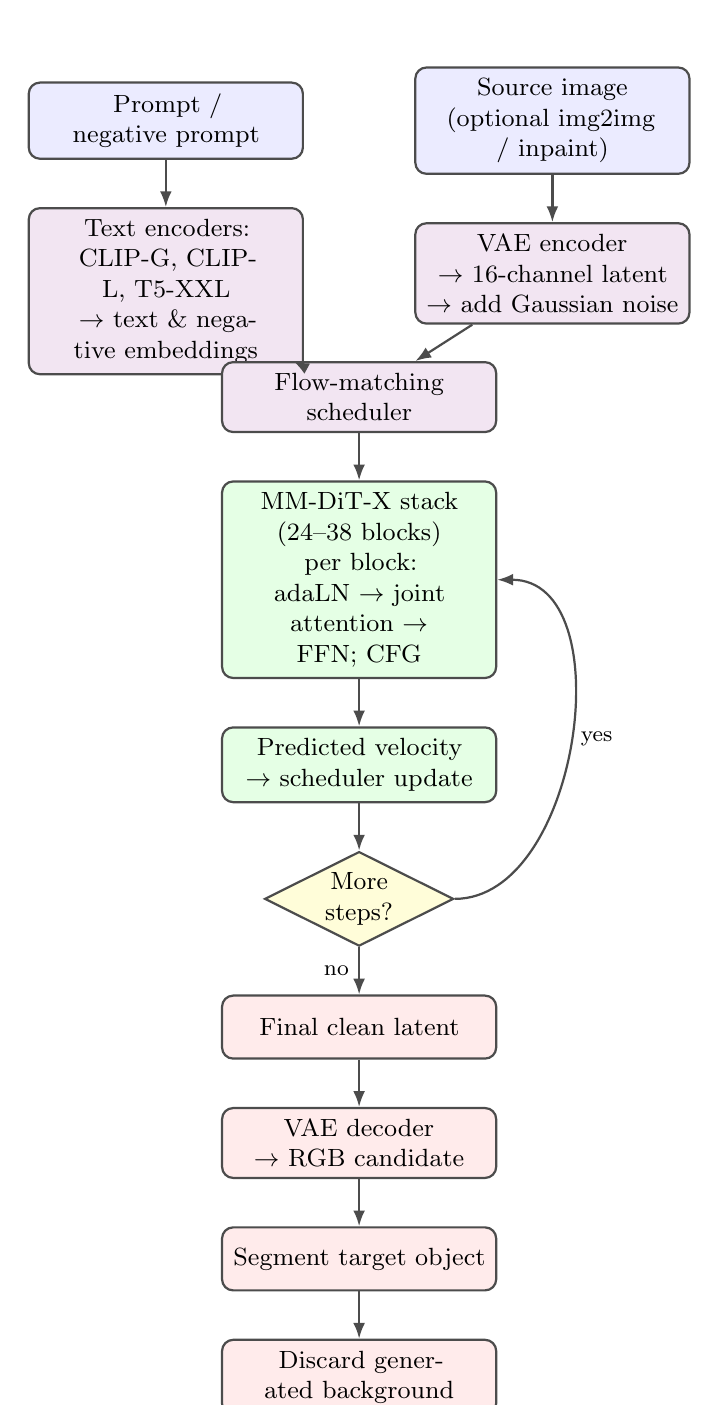
\begin{tikzpicture}[node distance=6mm and 14mm]
    \node[srcbox] (p)   {Prompt /\\negative prompt};
    \node[srcbox, right=of p] (src) {Source image\\(optional img2img / inpaint)};
    \node[genbox, below=of p]   (te)  {Text encoders:\\CLIP-G, CLIP-L, T5-XXL\\$\to$ text \& negative embeddings};
    \node[genbox, below=of src] (vae) {VAE encoder\\$\to$ 16-channel latent\\$\to$ add Gaussian noise};
    \coordinate (mid) at ($(te)!0.5!(vae)$);
    \node[genbox,  below=10mm of mid] (sch)  {Flow-matching scheduler};
    \node[compbox, below=of sch]      (dit)  {MM-DiT-X stack (24--38 blocks)\\per block: adaLN $\to$ joint\\attention $\to$ FFN; CFG};
    \node[compbox, below=of dit]      (vel)  {Predicted velocity\\$\to$ scheduler update};
    \node[decbox,  below=of vel]      (more) {More\\steps?};
    \node[validbox, below=of more]    (fin)  {Final clean latent};
    \node[validbox, below=of fin]     (dec)  {VAE decoder\\$\to$ RGB candidate};
    \node[validbox, below=of dec]     (seg)  {Segment target object};
    \node[validbox, below=of seg]     (disc) {Discard generated background};
    \draw[flowarr] (p) -- (te);
    \draw[flowarr] (src) -- (vae);
    \draw[flowarr] (te) -- (sch);
    \draw[flowarr] (vae) -- (sch);
    \draw[flowarr] (sch) -- (dit);
    \draw[flowarr] (dit) -- (vel);
    \draw[flowarr] (vel) -- (more);
    \draw[flowarr] (more) -- node[left,font=\footnotesize]{no} (fin);
    \draw[flowarr] (fin) -- (dec);
    \draw[flowarr] (dec) -- (seg);
    \draw[flowarr] (seg) -- (disc);
    \draw[flowarr] (more.east) to[out=0,in=0]
          node[right,font=\footnotesize]{yes} (dit.east);
  \end{tikzpicture}
  \caption[Generation flow]{The SD3.5 generation flow used inside the
  context/candidate generation step of every flow (re-drawn from
  \texttt{docs/diagram.md}). Text conditioning (the three encoders; T5-XXL
  disabled by default here) and an optionally img2img-encoded latent feed the
  flow-matching denoise loop over the MM-DiT-X stack; the final latent is decoded,
  the target object is segmented, and the generated background is discarded
  - the point at which background-as-source-of-truth begins.}
  \label{fig:genflow}
\end{figure}

\subsection{Dataset and split protocol}\label{sec:dataset}
The repository contains a broader data-engineering design than the saved experiment
archive. To avoid conflating a candidate source with data proven to have
been used in the reported adapter, this section distinguishes three roles:
(1) sources available to the ETL or rule-guided pipeline, (2) the concept-training
source stated for the saved LoRA configuration, and (3) source backgrounds visible
in the saved qualitative exports.

The reported concept-LoRA configuration identifies the person-class subset of
Paint-by-Inpaint / PIPE~\cite{pipe} as the generation-target source. PIPE contains
$888{,}000$ train and $752$ test items at $512\times512$ across $824$
\texttt{Instruction\_Class} categories. The loader is intended to retain only
whole-word person classes; the before/after pairing is not required for the plain
text-to-image concept objective. CityPersons~\cite{citypersons} supplies the
pedestrian reference domain and is visibly used for the saved Frankfurt/Aachen
composites. MOT17-02~\cite{mot17} and the human-detection collection are candidate
sources in the project data contract, but the saved report archive does not contain
a release manifest that proves their post-filter contribution to the LoRA artifact.

The intended split policy is group-aware: CityPersons by scene, MOT17 by sequence
window, and the human-detection collection by perceptual-duplicate cluster. The
CityPersons validation/test material should remain frozen for downstream evaluation
and must not be used for LoRA training, prompt tuning, threshold tuning, or synthetic
background selection. The current archive does not retain a complete release
manifest, post-filter counts, or the background-source provenance for every one of
the $100$ LoRA metric rows. Accordingly, this report does not claim that those
$100$ rows constitute a PIPE test-set evaluation or a fully verified CityPersons
benchmark.

\begin{table}[t]
  \centering
  \caption[Dataset roles and evidence status]{Dataset roles separated by what is
  defined in the project protocol versus what is retained in the saved report
  archive. ``Not retained'' means the report cannot independently substantiate the
  corresponding run-level contribution.}
  \label{tab:dataset}
  \small
  \begin{tabular}{@{}p{2.8cm}p{3.5cm}p{3.8cm}@{}}
    \toprule
    Source & Role in protocol & Evidence retained for this report \\
    \midrule
    CityPersons~\cite{citypersons} & Pedestrian reference domain; source backgrounds for rule-guided and qualitative composite examples; valid/test intended frozen benchmark. & Frankfurt/Aachen examples are present; per-row evaluation provenance is not retained. \\
    MOT17-02 & Candidate ETL source; group by sequence-time window. & Available in the data design; no post-filter contribution log retained. \\
    Human detection & Candidate positive/background source; group by perceptual cluster. & Available in the data design; no post-filter contribution log retained. \\
    PIPE~\cite{pipe} & Person-class generation targets for the stated concept-LoRA configuration. & Referenced by the configuration narrative; exact retained training count and release manifest are absent. \\
    \bottomrule
  \end{tabular}
\end{table}
\subsection{Recommended paired smoke-test protocol}\label{sec:smoke-plan}
A future controlled smoke test should use four source sets with ten source images per set, giving $40$ source scenes. Each scene can receive up to five candidate attempts, yielding a planned budget of
\begin{equation}
  4\ \text{source sets}\times 10\ \text{images per set}\times 5\ \text{attempts per image}=200\ \text{candidate attempts}.
\end{equation}
This $200$-candidate budget is a future validation design and is not reported as an observed sample size in this study. The retained archive instead provides three Rule-Guided summaries over $150$ candidates, a Rule-Guided shared-metric export with $32$ rows, and a LoRA shared-metric export with $100$ rows.

For a valid paired comparison, the evaluation set must be split before tuning. A small development subset may tune thresholds and image-processing controls, while the final $40$ source scenes remain frozen. Both flows should use the same source image, target prompt, seed where supported, detector version and threshold, output resolution, and effective-support mask convention. This protocol prevents different test conditions from being interpreted as a performance gain.

\subsection{Flow A - Rule-Guided SD3.5 Pipeline (Primary pipeline)}\label{sec:v5}
This report designates \rgp as the primary augmentation flow. It treats the MM-DiT backbone (\cref{sec:backbone}) as a black-box
img2img candidate generator and places all background-preservation
logic outside it. The motivating observation is architectural rather than
empirical: because rectified-flow denoising (\cref{eq:rf}) can in principle move
any latent token, no prompt or guidance setting guarantees that pixels
outside the intended object stay fixed - so \rgp never asks the model to
preserve them. Instead it generates a candidate, segments only the new
object, discards the generated background, and composites the object onto the
untouched source. The original image is the source of truth; generated
background pixels are never used as the final canvas outside the effective
composite support. The pipeline is a fixed sequence of
explicit stages:
\begin{equation}\label{eq:v5}
  \begin{aligned}
  &\text{placement}\to\text{context generation}\to\text{segmentation}\to\\
  &\text{scale correction}\to\text{compositing}\to\text{validation}\to\text{retry}.
  \end{aligned}
\end{equation}

\subsubsection*{Stages}
(1)~Placement proposes a valid insertion region from object-specific
priors (road or sidewalk masks, existing person/vehicle boxes, depth ordering,
overlap checks) - placement is a policy, not a prompt, since a realistic
object in an invalid location still corrupts the dataset.
(2)~Context generation runs SD3.5 img2img over a local context crop, so
the model has enough surrounding scene to produce a coherent, correctly-lit
candidate (the lesson from the V1--V4 ablations: too little canvas yields ghosts;
too much rewrites the scene).
(3)~Segmentation extracts the new object with YOLOv8m-seg.
(4)~Scale correction estimates expected pixel height from
depth/ground-position, resizes the crop and mask together with the contact point
(feet) anchored, and rejects objects outside a plausible size envelope -
geometry, not text, governs scale.
(5)~Compositing cleans the mask, trims the generated-background fringe,
applies occlusion rules against foreground persons/vehicles, harmonises
colour/brightness/texture/edge (optional contact shadow), and alpha-pastes only
the object pixels.
(6)~Validation + retry re-runs the detector and geometry/background
checks; weak samples are rejected and regenerated under a bounded budget rather
than saved.

\subsubsection*{Quality score and safety gate}
\rgp keeps a fused quality score as a flow-specific extension (not part of
the shared core of \cref{sec:metrics}):
\begin{equation}\label{eq:v5score}
  Q = 0.45\,s_{\text{obj}} + 0.25\,s_{\text{scale}}
    + 0.20\,s_{\text{bg}} + 0.10\,s_{\text{edge}},
\end{equation}
used for analysis and conservative autotune guidance, not as a claim of absolute
image quality. By policy augmentation is restricted to the \texttt{train} split
so it cannot contaminate the evaluation benchmark - \texttt{target\_splits}
is set to \texttt{train} only. \Cref{fig:v5arch} draws the staged flow of
\cref{eq:v5}, with the trusted-background path highlighted.

\subsubsection*{Tuning functions and safe parameter updates}
The Rule-Guided SD3.5 Pipeline exposes tuning controls so that a failed candidate can be diagnosed and improved without silently weakening the evaluation protocol. Tuning is performed only on a development subset. Once the final smoke set is frozen, parameters are fixed and no longer changed from one test image to the next.

\begin{table}[t]
  \centering
  \caption[Rule-guided tuning functions]{\textbf{Rule-guided tuning functions.} Each function changes a defined part of the pipeline and is linked to a recorded failure type. Exact values must be saved in the run configuration.}
  \label{tab:tuning-functions}
  \scriptsize
  \begin{tabular}{@{}p{2.25cm}p{3.05cm}p{3.15cm}p{1.15cm}@{}}
    \toprule
    \textbf{Function} & \textbf{Controls} & \textbf{Used when} & \textbf{Output} \\
    \midrule
    Placement tuning & Safe-region score, depth range, object clearance, foot-anchor location. & Bad placement or bad depth overlap. & Valid placement proposal or rejection. \\
    Context-generation tuning & Context crop margin, denoise strength, guidance scale, inference steps. & Candidate has poor local lighting, shape, or scene fit. & New candidate image. \\
    Mask tuning & Detection threshold, mask erosion, feather radius, small-component removal. & Mask aspect is invalid or the boundary has a halo. & Clean object mask. \\
    Geometry tuning & Expected-height envelope, scale correction, ground-contact tolerance. & Floating person or unrecoverable scale. & Resized crop and anchored mask, or rejection. \\
    Blend tuning & Colour matching and edge blending. & Visible seam or sticker effect. & Lower seam risk. \\
    Acceptance tuning & Quality-score threshold $\tau_Q$, component thresholds, maximum retries. & Candidate fails the final safety gate. & Accept, record reason, or retry. \\
    \bottomrule
  \end{tabular}
\end{table}

The flow-specific quality score in \cref{eq:v5score} is used to rank or reject candidates after the required hard checks. A safe tuning rule is
\begin{equation}\label{eq:tuning}
\begin{aligned}
  \theta^* &= \arg\max_{\theta\in\Theta}\ \frac{1}{|D_{\mathrm{dev}}|}\sum_{x\in D_{\mathrm{dev}}}Q(x;\theta), \\
  &\text{subject to a fixed benchmark split, detector, and acceptance policy on }D_{\mathrm{test}}.
\end{aligned}
\end{equation}
Here $\theta$ contains the tunable controls in \cref{tab:tuning-functions}. The constraint is important: it prevents the final smoke set from becoming a tuning set.

\begin{figure}[H]
  \centering
  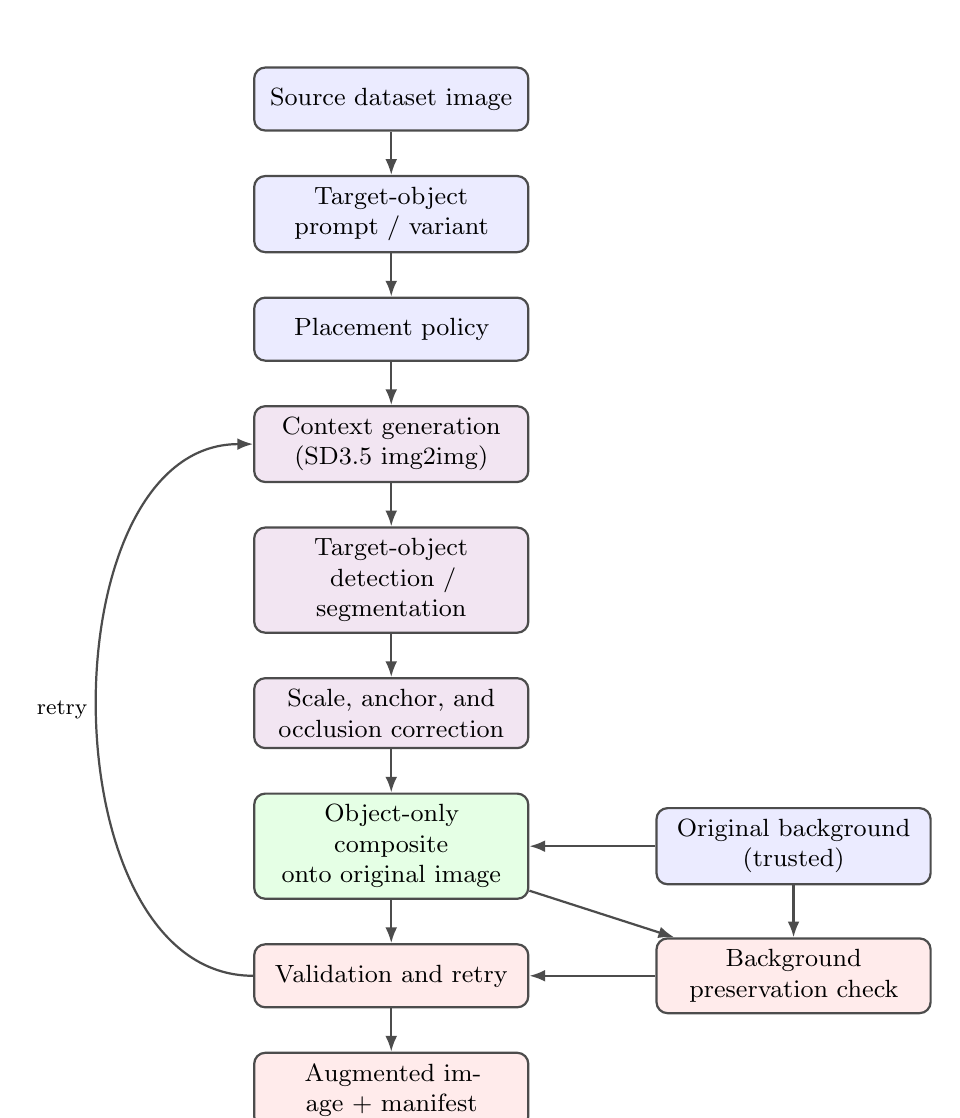
\begin{tikzpicture}[node distance=5.5mm and 16mm]
    \node[srcbox]            (a) {Source dataset image};
    \node[srcbox, below=of a](b) {Target-object prompt / variant};
    \node[srcbox, below=of b](c) {Placement policy};
    \node[genbox, below=of c](d) {Context generation\\(SD3.5 img2img)};
    \node[genbox, below=of d](e) {Target-object detection /\\segmentation};
    \node[genbox, below=of e](f) {Scale, anchor, and\\occlusion correction};
    \node[compbox, below=of f](g) {Object-only composite\\onto original image};
    \node[validbox, below=of g](h) {Validation and retry};
    \node[validbox, below=of h](i) {Augmented image + manifest};
    % trusted-background side path
    \node[srcbox, right=of g] (j) {Original background\\(trusted)};
    \node[validbox, right=of h] (k) {Background\\preservation check};
    \draw[flowarr] (a)--(b);
    \draw[flowarr] (b)--(c);
    \draw[flowarr] (c)--(d);
    \draw[flowarr] (d)--(e);
    \draw[flowarr] (e)--(f);
    \draw[flowarr] (f)--(g);
    \draw[flowarr] (g)--(h);
    \draw[flowarr] (h)--(i);
    \draw[flowarr] (j)--(g);
    \draw[flowarr] (j)--(k);
    \draw[flowarr] (g)--(k);
    \draw[flowarr] (k)--(h);
    \draw[flowarr] (h.west) to[out=180,in=180]
          node[left,font=\footnotesize]{retry} (d.west);
  \end{tikzpicture}
  \caption[Rule-Guided SD3.5 Pipeline architecture]{The \rgp context--object composite
  flow of \cref{eq:v5} (re-drawn from \texttt{docs/diagram.md}). The blue
  original background is the trusted source: it is composited under the
  segmented object and is the reference for the background-preservation check, so
  pixels outside the effective composite support are never taken from generation.
  Failed validations retry the generation stage under a bounded budget.}
  \label{fig:v5arch}
\end{figure}

\subsection{Flow B - Concept LoRA + segment-and-paste (Auxiliary flow)}\label{sec:lora}
\textsc{LoRA} is retained as an auxiliary concept-generation flow rather than the primary augmentation path. It separates the two responsibilities that the harder mask-free
edit variant conflated: what to generate (learned by a LoRA) and
which pixels to keep (enforced by construction at paste time). The
current flow takes the simpler of the two paths - it learns to generate
people, not to edit a given scene - and then recovers the background by the
same segment-and-composite principle as \rgp.
Implementation note: an earlier mask-free edit LoRA conditioned the
denoiser on a source latent (an InstructPix2Pix-style~\cite{ip2p} image path with
a trainable input projection and two-scale CFG) was prototyped but retired; the
flow in the repository today is the plain text$\to$image concept LoRA described
here, with segment-and-paste as the compositing step.

\subsubsection*{Training: a plain text$\to$image concept LoRA}
A single LoRA is trained, DreamBooth-style, so the frozen SD3.5 backbone learns to
generate images in the distribution of the PIPE ``add a person'' subset.
There is no mask, no source image, and no image-conditioning projection: training
is the standard SD3 rectified-flow objective on the target latent alone,
\begin{equation}\label{eq:lora-cond}
  z_t = (1-\sigma_t)\,z_{\text{img}} + \sigma_t\,\epsilon,\qquad
  \mathcal{L} = w(\sigma_t)\,\big\lVert \hat v_\theta(z_t,t,c_{\text{text}})
  - (\epsilon - z_{\text{img}}) \big\rVert^2 ,
\end{equation}
where $z_{\text{img}}=\text{VAE}(\text{image})$ and $c_{\text{text}}$ is the
precomputed text embedding. Only the attention LoRA adapters are trained; the
MM-DiT weights and the three text encoders stay frozen, and text embeddings are
precomputed to disk so the encoders can be dropped during the T4-budget run
(bf16 compute, fp32 trainable). Inference therefore needs a single artifact -
\texttt{adapter/pytorch\_lora\_weights.safetensors} - and no input projection.

\subsubsection*{Why PIPE images}
The concept LoRA is trained on the person-class subset of PIPE~\cite{pipe}: real
photographs that contain people, used as plain generation targets (the
before/after pairing that PIPE was built for is not needed here, since the LoRA
generates rather than edits). The loader filters strictly on the
\texttt{Instruction\_Class} field (whole-word person classes; the free-text
caption is never matched, so a non-person image cannot leak in). Of PIPE's
$888{,}000$ images only the person-class subset is retained (the exact count is
logged by the loader at train time).

\subsubsection*{Generate $\to$ segment $\to$ paste}
Background preservation is an inference-time composite, not a training objective:
\begin{enumerate}[leftmargin=1.6em,itemsep=2pt]
  \item Generate. Base SD3.5 + the trained LoRA run the standard
        rectified-flow denoise loop from the prompt alone, producing a full image
        that contains a person. The model never sees the original scene, so
        the generated background is its own - not the target's.
  \item Segment. YOLOv8-seg (COCO class~0) returns a per-person
        $\{\text{mask},\text{bbox},\text{conf}\}$ from the generated frame; low-confidence
        or tiny detections are dropped.
  \item Paste. The segmented person is composited onto the
        original background. The mask is eroded a pixel or two to drop the
        YOLO background halo, the alpha is feathered for a soft seam, and a
        Reinhard colour transfer shifts the person's per-channel mean/std toward
        the pixels it covers (optional OpenCV Poisson \texttt{seamlessClone} for
        the largest person). The intended final canvas outside the effective composite support comes from
        the original image - a composite, not a learned or hard-restore
        approximation. Whether this is byte-exact after export must be verified
        separately with a pixel-level regression check.
\end{enumerate}
Known trade-off: the pasted person was lit by the generated scene,
so a paste can read as a sticker; mitigations are to raise the colour-match
strength or enable Poisson blending. The flow does not control where the
person lands (the prompt-only generator gives no placement prior), which is the
price of the simpler concept-LoRA path relative to a scene-conditioned editor
such as FLUX.1 Kontext~\cite{kontext} - the latter keeps the edit in one model
pass but gives no source-image composite constraint outside the retained
support, the property this flow prioritises.

\begin{figure}[H]
  \centering
  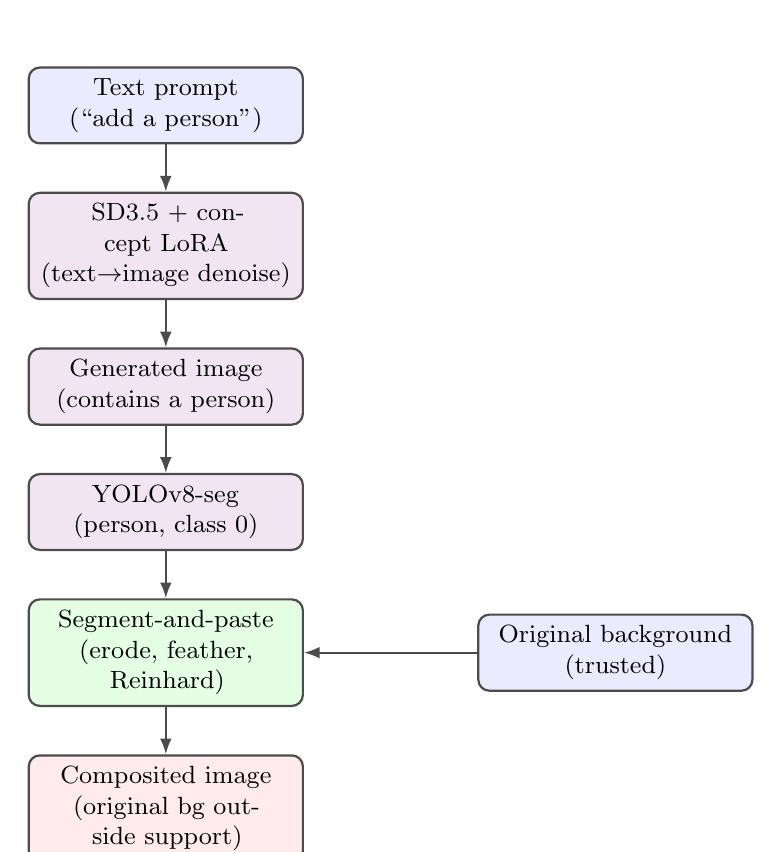
\begin{tikzpicture}[node distance=6mm and 14mm]
    \node[srcbox]              (txt) {Text prompt\\(``add a person'')};
    \node[genbox, below=of txt](gen) {SD3.5 + concept LoRA\\(text$\to$image denoise)};
    \node[genbox, below=of gen](img) {Generated image\\(contains a person)};
    \node[genbox, below=of img](seg) {YOLOv8-seg\\(person, class~0)};
    \node[compbox, below=of seg](paste){Segment-and-paste\\(erode, feather,\\Reinhard)};
    \node[validbox, below=of paste](out){Composited image\\(original bg outside support)};
    % trusted-background side path
    \node[srcbox, right=22mm of paste] (orig) {Original background\\(trusted)};
    \draw[flowarr] (txt)--(gen);
    \draw[flowarr] (gen)--(img);
    \draw[flowarr] (img)--(seg);
    \draw[flowarr] (seg)--(paste);
    \draw[flowarr] (paste)--(out);
    \draw[flowarr] (orig)--(paste.east);
  \end{tikzpicture}
  \caption[LoRA flow]{The \textsc{LoRA} concept-generate-then-paste flow
  (\cref{sec:lora}). A concept LoRA generates a person from the prompt alone; the
  person is segmented and composited onto the trusted original background, so the
  generated background is discarded and the final canvas outside the effective
  composite support is sourced from the original image.}
  \label{fig:loraarch}
\end{figure}

\subsection{Two flows with different output types}\label{sec:selection}
The two flows use the same broad idea: generate a person, keep only the person support, and place that support on the source image. They differ in what is generated, what is controlled, and what image is exported. The study keeps their outputs separate so that an accepted rule-guided training image is not confused with a LoRA appearance sample.

\begin{table}[t]
  \centering
  \caption[Two output types]{\textbf{Two image types produced by the study.} The two outputs are stored and interpreted separately because their generation inputs and validation rules are different.}
  \label{tab:two-output-types}
  \scriptsize
  \begin{tabular}{@{}p{2.75cm}p{2.65cm}p{2.8cm}p{2.35cm}@{}}
    \toprule
    \textbf{Output type} & \textbf{Generation input} & \textbf{What is kept in the final image} & \textbf{Use in this report} \\
    \midrule
    Rule-guided accepted composite & Source scene, local context crop, target prompt, placement proposal. & A scene-aware pedestrian crop pasted on the original source image after validation and retry. & Main controlled-augmentation output. \\
    LoRA segment-and-paste composite & Text prompt for a person, then a separate source background for paste. & A prompt-generated person crop pasted on the original source image. & Auxiliary appearance-generation output and metric baseline. \\
    \bottomrule
  \end{tabular}
\end{table}

The rule-guided flow observes local scene context before candidate generation and then applies placement, depth, scale, grounding, occlusion, validation, and retry controls. The concept LoRA flow generates a person from text alone. It is useful for studying learned pedestrian appearance, but target-scene placement and expected scale are not defined in the exported LoRA experiment. The raw metric comparison is presented first in \cref{sec:rawmetrics}; the final method-selection decision is made later in \cref{sec:decision}.

\subsection{Shared metric core}\label{sec:metrics}
Both flows use a dependency-injected metric module built from NumPy, Pillow, and
an injected detector callable. The module is useful only when each metric is read
according to what it actually measures:
\begin{itemize}[leftmargin=1.4em,itemsep=2pt]
  \item Detection. \textsc{person\_detected} and
        \textsc{person\_confidence} state whether any person is detected
        in the output. In crowded CityPersons images this is not target-specific,
        because source pedestrians can keep the flag positive even when insertion
        fails.
  \item Inclusion. \textsc{inclusion\_count\_delta} equals output person
        count minus source person count. In the supplied LoRA CSV,
        \textsc{object\_added} is exactly $\mathbb{1}[\Delta n>0]$ for every row.
        This is a useful proxy, but it should ultimately be replaced or augmented
        by target-mask / target-box overlap.
  \item Scale. \textsc{scale\_ratio} and \textsc{scale\_error} require
        a non-zero expected-height prior. A missing prior must remain missing; it
        must not be encoded as a perfect score.
  \item Background preservation. \bgmae and \bgssim are computed outside
        implementation-defined effective support $M_{\mathrm{eff}}$. A value close
        to zero / one measures low change under that convention, not automatically
        byte-exact preservation. A separate pixel-regression assertion is required
        for the latter claim.
\end{itemize}

\begin{table}[t]
  \centering
  \caption[Metric interpretation]{Metric interpretation used in this report.
  Detector presence and count delta are proxies; they do not prove that the
  detector found the newly inserted target.}
  \label{tab:shared-metrics}
  \small
  \begin{tabular}{@{}p{3.6cm}p{5.2cm}p{1.6cm}@{}}
    \toprule
    Metric & Interpretation & Direction \\
    \midrule
    \textsc{person\_detected} / \textsc{person\_confidence} & Any person detected in output; not target-specific in multi-person scenes. & higher \\
    \textsc{object\_added} / \textsc{inclusion\_count\_delta} & Detector-count evidence for a new person relative to source; needs target-overlap confirmation. & higher \\
    \textsc{scale\_ratio} / \textsc{scale\_error} & Detected versus expected height, only when expected height is non-zero. & ratio neutral; error lower \\
    \bgmae / \bgssim & Difference outside a common $M_{\mathrm{eff}}$ support convention. & MAE lower; SSIM higher \\
    \bottomrule
  \end{tabular}
\end{table}

\subsection{Evaluation protocol and LoRA audit}\label{sec:protocol}
A valid paired comparison would require the same frozen source cases, prompts,
seeds, detector version and threshold, common effective-support masks, and common
output format for both flows. The supplied archive does not contain those matched
rule-guided per-case metrics. It instead contains three rule-guided smoke summaries
and one $N=100$ LoRA shared-metric CSV. The report first reports the raw shared metrics as they are exported. It then makes a separate operational method-selection decision based on the controls required for safe pedestrian insertion. It does not claim an unpaired cross-flow effect size for background or inclusion metrics.

The LoRA CSV was audited programmatically before aggregation. It contains $100$
rows, all labelled \texttt{lora}, with $100$ unique \textsc{case\_id} values and
$100$ unique seeds from $42$ through $141$. No values are missing in detection,
inclusion, or background columns. The arithmetic identity
\textsc{person\_count}$-$\textsc{source\_person\_count}$=$\textsc{inclusion\_count\_delta}
holds in every row, and \textsc{object\_added} equals $\mathbb{1}[\Delta n>0]$ in
every row. In contrast, \textsc{expected\_height} equals $0$ in all rows and both
scale columns are missing in all rows. Thus, the inclusion and background statistics
are usable under their stated conventions, whereas LoRA scale performance is not
measurable from this export.

The project code identifies YOLOv8~\cite{yolov8} as the detector family (YOLOv8n
for detection and YOLOv8m-seg where masks are needed), using a default confidence
threshold of $0.25$ and an $8$\,px dilation before background metrics. These
settings are recorded as code defaults; run-level model and configuration hashes
remain required for a fully reproducible benchmark.
% ============================================================================
\section{Results and Discussion}\label{sec:results}

\subsection{Raw shared-metric comparison}\label{sec:rawmetrics}
The supplied shared-metric files do not support a paired performance claim. The Rule-Guided file contains $32$ rows with $31$ unique case IDs and $32$ unique case--seed pairs. The LoRA file contains $100$ unique case IDs and $100$ unique case--seed pairs. The source scenes, output provenance, and effective-support masks are not matched. The values below are therefore reported as raw observations, not as a statistically valid head-to-head benchmark.

\begin{table}[t]
  \centering
  \caption[Raw shared-metric comparison]{\textbf{Raw shared-metric comparison from the supplied CSV files.} Bold text identifies the higher or lower raw value where a direction exists; it does not establish a fair cross-flow winner because the runs are unpaired.}
  \label{tab:raw-shared-comparison}
  \scriptsize
  \begin{tabular}{@{}p{2.85cm}p{2.1cm}p{2.1cm}p{3.35cm}@{}}
    \toprule
    \textbf{Metric} & \textbf{Rule-Guided ($N=32$)} & \textbf{LoRA ($N=100$)} & \textbf{Reading} \\
    \midrule
    Object-added rate & $18/32=0.563$ & \textbf{$69/100=0.690$} & LoRA is higher in the exported detector-count proxy. \\
    Mean count delta & $0.469$ & \textbf{$0.720$} & LoRA is higher in the exported detector-count proxy. \\
    Mean person confidence & \textbf{$0.894$} & $0.851$ & Rule-Guided is higher, but this is not target-specific in crowded scenes. \\
    Mean background MAE & $19.108$ & \textbf{$0.212$} & LoRA is lower under its own exported support convention. \\
    Mean background SSIM & $0.554$ & \textbf{$0.997$} & LoRA is higher under its own exported support convention. \\
    Scale error & Not available & Not available & Expected height is zero and scale fields are empty in both shared-metric CSVs. \\
    \bottomrule
  \end{tabular}
\end{table}

The raw metric table gives LoRA the numeric lead for addition rate, count delta, and the two background metrics. This finding must be stated plainly. It does not show that LoRA is the better controlled-augmentation system because the metrics are calculated on different output sets and do not measure placement correctness, grounding, occlusion correctness, or target-specific scale. The Rule-Guided shared file also has a wide background range: mean \bgmae $19.108$ (SD $13.341$; min $1.173$; max $35.851$) and mean \bgssim $0.554$ (SD $0.356$; min $0.135$; max $0.996$). This requires a common-mask audit before background values are used for a final method ranking.

\subsubsection*{LoRA metric audit}
The LoRA CSV was audited rather than reported from its mean values alone. It contains $100$ rows, $100$ unique cases, and $100$ unique seeds. Object addition is $69/100=0.690$ with a 95\% Wilson interval $[0.594,0.772]$. Mean inclusion-count delta is $0.720$; the split is $69$ positive, $23$ zero, and $8$ negative rows. The $98/100$ person-detection rate is not target-specific because source pedestrians can keep the detector positive when no new pedestrian is added.

LoRA background values are favourable on average: mean \bgmae $0.2120$ (SD $1.1374$, median $0$, P95 $0.8588$, maximum $10.6237$) and mean \bgssim $0.9969$ (SD $0.0177$, median $1.0000$, minimum $0.8329$). However, $20$ rows have non-zero \bgmae, $4$ exceed $1.0$, and $5$ have \bgssim below $0.99$. The correct statement is low average background change under the exported support convention, not a universal guarantee of unchanged pixels. LoRA scale remains unevaluable because expected height is zero in all $100$ rows and both scale columns are missing.

\begin{table}[t]
  \centering
  \caption[Audited LoRA shared metrics]{\textbf{LoRA metric audit.} The audit keeps uncertainty and failure counts visible instead of reporting only a single mean.}
  \label{tab:lora-audit}
  \scriptsize
  \begin{tabular}{@{}p{2.55cm}p{3.6cm}p{3.55cm}@{}}
    \toprule
    \textbf{Area} & \textbf{Audited result} & \textbf{Interpretation} \\
    \midrule
    Row integrity & $100$ rows; $100$ unique cases; $100$ unique seeds ($42$--$141$). & No duplicate row identity or mixed-flow label. \\
    Object addition & \textbf{$69/100=0.690$}; 95\% Wilson $[0.594,0.772]$. & \textsc{object\_added} matches $\Delta n>0$. \\
    Count delta & Mean $0.720$; $69/23/8$ positive/zero/negative. & Detector-count proxy; negative rows require review. \\
    Person detection & $98/100=0.980$. & Not target-specific: source people can keep this value positive. \\
    Person confidence & Mean $0.851$, SD $0.149$; detected-only mean $0.868$. & Includes two zero-confidence rows. \\
    Background MAE & \textbf{Mean $0.2120$}; max $10.6237$; $80$ zero rows. & Strong central value with visible outliers. \\
    Background SSIM & \textbf{Mean $0.9969$}; min $0.8329$; $85$ rows equal $1.0$. & Strong average similarity, not a bit-exact proof. \\
    Scale & No valid scale rows. & Expected height is zero and scale fields are missing. \\
    \bottomrule
  \end{tabular}
\end{table}

\subsection{Rule-guided primary-pipeline diagnostics}\label{sec:ablation}
\Cref{tab:v5summary} aggregates the three saved \rgp metric summaries. Their exact source/run mapping is recorded in the reproducibility statement: \nolinkurl{metrics_summary.csv} maps to cityperson\allowbreak\_nguyena, \nolinkurl{metrics_summary (1).csv} maps to cityperson\allowbreak\_bg\allowbreak\_yolo, and \nolinkurl{metrics_summary (2).csv} maps to \texttt{MOT17}. Across these smoke runs, $150$ candidates were generated, $103$ accepted, and $47$ rejected, yielding a weighted acceptance rate of $0.687$.

The accepted proportion improves from $0.60$ on cityperson\allowbreak\_nguyena to
$0.72$ on cityperson\allowbreak\_bg\allowbreak\_yolo and $0.74$ on \texttt{MOT17}. The
reported flow-specific scale score is $0.9676$, $0.9742$, and $0.9284$,
respectively; its aggregate $0.957$ is the unweighted mean of the three run-level
means, not a pooled per-candidate statistic. While the saved summaries do not
contain the shared background / inclusion fields, they demonstrate that the primary
flow operationalises the constraints absent from the LoRA export: a candidate is
saved only after its placement and geometry checks pass.

\Cref{tab:rejecthist} shows that \texttt{mask\_aspect\_invalid} is the dominant
rejection category ($28/47$, $59.6\%$), followed by \texttt{bad\_placement}
($11/47$, $23.4\%$). The result directs future work toward segmentation and
placement-policy refinement, not a relaxation of quality gates. The rejected
examples are useful diagnostics rather than evidence that the filter should accept
weaker samples.

\begin{table}[t]
  \centering
  \caption[Rule-guided primary-flow diagnostics]{Three saved source/run-specific
  \rgp smoke summaries. Aggregate acceptance is total accepted / total generated;
  the aggregate scale value is the unweighted mean of the three run-level means.}
  \label{tab:v5summary}
  \scriptsize
  \begin{tabular}{@{}lrrrrr@{}}
    \toprule
    Source/run & Generated & Accepted & Rejected & Accept rate & Mean scale \\
    \midrule
    cityperson\allowbreak\_nguyena & 50 & 30 & 20 & 0.60 & 0.9676 \\
    cityperson\allowbreak\_bg\allowbreak\_yolo & 50 & 36 & 14 & 0.72 & 0.9742 \\
    \texttt{MOT17} & 50 & 37 & 13 & 0.74 & 0.9284 \\
    \midrule
    Aggregate (three runs) & 150 & 103 & 47 & 0.687 & 0.957 \\
    \bottomrule
  \end{tabular}
\end{table}

\begin{table}[t]
  \centering
  \caption[Aggregated rule-guided rejection histogram]{Aggregated rejection
  histogram across the three supplied \rgp smoke summaries
  ($N_{\mathrm{rejected}}=47$). Reason labels are preserved from the CSV fields.}
  \label{tab:rejecthist}
  \scriptsize
  \begin{tabular}{@{}lrr@{}}
    \toprule
    Reject reason & Count & Share of rejected \\
    \midrule
    \texttt{mask\_aspect\_invalid} & 28 & 0.596 \\
    \texttt{bad\_placement} & 11 & 0.234 \\
    \texttt{bad\_person\_depth\_overlap} & 3 & 0.064 \\
    \texttt{floating\_or\_bad\_ground} & 2 & 0.043 \\
    \texttt{scale\_unrecoverable} & 2 & 0.043 \\
    \texttt{no\_person\_detected} & 1 & 0.021 \\
    \midrule
    Total & 47 & 1.000 \\
    \bottomrule
  \end{tabular}
\end{table}


\subsection{Recommended blinded manual review for future confirmation}\label{sec:manualreview}
The automated metrics do not establish whether an inserted pedestrian is physically plausible in its target scene. In particular, they do not directly measure safe placement, scale and ground contact, foreground occlusion, or whether the final image is appropriate for detector training. No blinded manual-review scores were supplied with the archive; therefore, no manual-review result is reported in this study.

A future review should use the $40$ frozen source scenes specified in \cref{sec:smoke-plan}. For each source scene, one final Rule-Guided output and one final LoRA output should be anonymised, randomly ordered, and shown without flow names, paths, prompts, metric values, or debug overlays. At least three independent reviewers should score visual realism, scene compatibility, placement plausibility, scale and grounding, boundary quality, and usefulness for dataset augmentation on a $1$--$5$ scale. Each reviewer should also assign a binary augmentation-ready decision.

For image $i$ and reviewer $r$, the per-image score may be computed as
\begin{equation}\label{eq:manualscore}
S_{i,r}=\frac{1}{6}\sum_{k=1}^{6}s_{i,r,k}, \qquad s_{i,r,k}\in\{1,2,3,4,5\}.
\end{equation}
The future report should provide the method-level mean, augmentation-ready rate, paired source-scene win/tie/loss counts, a paired Wilcoxon test, and reviewer agreement for the binary ready label using Fleiss' $\kappa$. A visual-superiority claim is justified only after these scores have been collected and retained as an auditable CSV.

\subsection{Operational decision: Rule-Guided SD3.5 Pipeline is the main flow}\label{sec:decision}
The raw shared metrics give LoRA the numeric lead on the currently exported addition and background values. This result is retained in the report and is not hidden. The primary-flow decision asks a different engineering question: which flow provides the scene-dependent controls required to produce controlled pedestrian augmentation? The selection below is based on implemented capabilities and retained Rule-Guided acceptance and rejection records; it is not a claim of measured visual superiority.

\begin{table}[t]
  \centering
  \caption[Method-selection decision]{\textbf{Method-selection decision after the raw metric comparison.} Rule-Guided is selected for the main pipeline because it covers the scene-dependent checks required by the task.}
  \label{tab:method-decision}
  \scriptsize
  \begin{tabular}{@{}p{3.0cm}p{2.9cm}p{2.9cm}p{1.1cm}@{}}
    \toprule
    \textbf{Required capability} & \textbf{Rule-Guided} & \textbf{LoRA} & \textbf{Choice} \\
    \midrule
    Uses target-scene context before generation & Local context crop. & Prompt-only person generation. & Main \\
    Places person in a safe region & Placement policy, depth, overlap, and clearance checks. & No target-scene placement policy in the export. & Main \\
    Checks scale and ground contact & Expected-height correction, foot anchor, and rejection. & No expected height or reported scale result. & Main \\
    Checks occlusion and invalid output & Occlusion rules, safety gate, rejection label, bounded retry. & Segment and paste; no comparable gate log. & Main \\
    Produces a retained operational quality log & $103/150$ accepted, $47$ rejected with reasons, mean scale score $0.957$. & $100$ shared-metric rows; no scale quality result. & Main \\
    Raw addition/background metric lead & Not present in the unpaired CSVs. & Higher raw addition and background values. & LoRA \\
    \bottomrule
  \end{tabular}
\end{table}

\begin{quote}
``Final operating decision: use the Rule-Guided SD3.5 Pipeline as the main dataset-augmentation flow and retain LoRA as a secondary appearance-generation baseline. LoRA currently has stronger raw shared-metric values. Rule-Guided is selected because it provides the scene-aware controls and rejection mechanisms required by the training-data task. This selection does not claim visual superiority without a paired evaluation and blinded review.''
\end{quote}

The saved Rule-Guided summaries support this decision. Across three smoke runs, the pipeline generated $150$ candidates, accepted $103$, and rejected $47$; the weighted acceptance rate is $0.687$ with a 95\% Wilson interval $[0.609,0.755]$. The mean scale score is $0.957$ across the three run-level means. Rejection is informative: invalid mask shape accounts for $28/47$ rejects and bad placement for $11/47$. These failure labels directly drive the tuning functions in \cref{tab:tuning-functions}. A production pipeline should reject unsafe samples rather than convert every detector-visible output into training data.

\subsection{Compute accounting: evidence gap}\label{sec:efficiency}
The archive supports only a qualitative implementation-cost description, not a
measured efficiency comparison. The rule-guided path performs placement proposal,
local img2img, segmentation, scale correction, validation, and bounded retries at
inference. The LoRA path pays a one-off adapter-training cost, then uses
text-to-image generation and YOLOv8-seg paste at inference; the saved adapter file
is reported as $29.1$\,MB. Because no per-case wall-clock, retry, throughput, or
peak-memory logs are retained, neither runtime nor VRAM is treated as a numerical
result. A future report should measure candidate time, accepted-output time,
retries, peak allocated VRAM, and energy/cost on the same hardware and seeds.
\subsection{Qualitative results}\label{sec:qual}
\Cref{fig:qual} provides illustrative saved outputs rather than a paired human
study. The upper examples are Type~A rule-guided accepted composites and the lower examples are Type~B LoRA segment-and-paste composites. The two image types must remain separate in the archive, figures, and training-data manifests. They should be inspected for paste-seam
sharpness, sticker-lighting, and local scale plausibility. They reinforce the role distinction visible in the workflow diagrams: Rule-Guided SD3.5 Pipeline is the scene-aware controlled-augmentation method, whereas LoRA is a prompt-only appearance generator followed by paste. They do not provide a paired numerical margin, so a final experiment report should replace them with enlarged matched source--candidate--mask--composite--difference panels.
\begin{figure}[t]
  \centering
  \begin{tabular}{@{}c@{ }c@{ }c@{} }
    \maybeincludegraphics[width=0.32\textwidth]{../../LoRA/notebooks/run_version/000017_pair_0006_add_occluded_pedestrian.png} &
    \maybeincludegraphics[width=0.32\textwidth]{../../LoRA/notebooks/run_version/000137_pair_0035_add_single_pedestrian.png} &
    \maybeincludegraphics[width=0.32\textwidth]{../../LoRA/notebooks/run_version/aachen_000008_000019_leftImg8bit_png_jpg.rf.f01332c4be688f6c98ad94d31395d5bc_pair_0011_add_occluded_pedestrian.png} \\
    \maybeincludegraphics[width=0.32\textwidth]{../../LoRA/notebooks/run_version/aachen_000057_000019_leftImg8bit_pair_0031_add_single_pedestrian.png} &
    \maybeincludegraphics[width=0.32\textwidth]{../../LoRA/notebooks/run_version/aachen_000066_000019_leftImg8bit_png_jpg.rf.67715c6432b08ab3ff35aed757a21496_pair_0037_add_distant_pedestrian.png} &
    \maybeincludegraphics[width=0.32\textwidth]{../../LoRA/notebooks/run_version/aachen_000153_000019_leftImg8bit_pair_0035_add_single_pedestrian.png} \\
  \end{tabular}

  \vspace{0.6em}

  \begin{tabular}{@{}c@{ }c@{ }c@{} }
    \maybeincludegraphics[width=0.32\textwidth]{../../LoRA/notebooks/run_version/concept_segpaste_export/concept_segpaste/images/frankfurt_000000_000294_leftImg8bit_segpaste.png} &
    \maybeincludegraphics[width=0.32\textwidth]{../../LoRA/notebooks/run_version/concept_segpaste_export/concept_segpaste/images/frankfurt_000000_000576_leftImg8bit_segpaste.png} &
    \maybeincludegraphics[width=0.32\textwidth]{../../LoRA/notebooks/run_version/concept_segpaste_export/concept_segpaste/images/frankfurt_000000_001016_leftImg8bit_segpaste.png} \\
    \maybeincludegraphics[width=0.32\textwidth]{../../LoRA/notebooks/run_version/concept_segpaste_export/concept_segpaste/images/frankfurt_000000_001236_leftImg8bit_segpaste.png} &
    \maybeincludegraphics[width=0.32\textwidth]{../../LoRA/notebooks/run_version/concept_segpaste_export/concept_segpaste/images/frankfurt_000000_001751_leftImg8bit_segpaste.png} &
    \maybeincludegraphics[width=0.32\textwidth]{../../LoRA/notebooks/run_version/concept_segpaste_export/concept_segpaste/images/frankfurt_000000_002196_leftImg8bit_segpaste.png} \\
  \end{tabular}
  \caption[Illustrative qualitative outputs]{\textbf{Two output types shown separately.} The upper rows are Type~A rule-guided accepted composites. The lower rows are Type~B LoRA prompt-generated person composites. The panels are not matched pairs and do not quantify a cross-flow gap.}
  \label{fig:qual}
\end{figure}

\subsection{Discussion}\label{sec:discussion}
The result has two parts and both must remain visible. First, LoRA has better raw values in the current shared-metric files for object-added rate, count delta, background MAE, and background SSIM. Second, those values do not answer whether a new pedestrian was placed at a safe position, at a valid scale, on the ground, behind or in front of the correct objects, or after a controlled retry process. The files are unpaired and their support-mask provenance is not the same, so direct numerical ranking would be misleading.

Rule-Guided SD3.5 Pipeline is selected as the main flow because the task is controlled data augmentation, not only person appearance generation. The pipeline sees local scene context, proposes a place, corrects scale, anchors the feet, checks occlusion, rejects invalid outputs, and records why a sample failed. The $103/150$ acceptance result and the rejection histogram show that these controls are active. LoRA remains useful because its current outputs have strong raw background numbers and a higher detector-count addition rate; it should be used as an appearance baseline and as a candidate source for future hybrid methods.

The final $40$-scene, $200$-candidate smoke run should make this selection testable on common conditions. The same frozen scenes, prompt variants, mask convention, detector version, threshold, and output format must be used for both flows. Each output should be matched to its intended insertion region. The report should then compare target-specific inclusion, scale error, placement score, grounding success, occlusion correctness, background change, time per accepted image, retries, and downstream detector benefit.

\section{Conclusion and Perspective}\label{sec:conclusion}
This study documents two distinct ways to create pedestrian training images while preserving the source background. Rule-Guided SD3.5 Pipeline generates a scene-conditioned candidate and saves it only after placement, scale, grounding, occlusion, and quality checks. The LoRA flow generates a person from text and pastes that person onto a source image. The two outputs are different products and are reported separately.

The current raw shared-metric CSVs favour LoRA for object-added rate ($0.690$ versus $0.563$), mean count delta ($0.720$ versus $0.469$), background MAE ($0.212$ versus $19.108$), and background SSIM ($0.997$ versus $0.554$). Rule-Guided has higher mean person confidence ($0.894$ versus $0.851$). These values cannot support a fair head-to-head ranking because the exported runs are unpaired, use different output cases, and do not retain common effective-support-mask provenance. Neither export contains valid shared scale-error data.

Rule-Guided SD3.5 Pipeline is nevertheless selected as the primary controlled-augmentation method for this project. This selection is supported by its implemented target-scene controls and by the retained operational smoke summaries: $103/150$ accepted candidates, weighted acceptance $0.687$, unweighted mean run-level scale score $0.957$, and explicit failure records. The two dominant failures are invalid mask shape ($28/47$) and bad placement ($11/47$); both are actionable through the tuning functions described in \cref{tab:tuning-functions}. LoRA remains a valuable secondary appearance baseline because it achieves strong raw addition and background values, but the supplied evidence does not demonstrate placement, grounding, occlusion, or scale assurance for that flow.

\subsection*{Final conclusion}
\begin{quote}
``For the current project, Rule-Guided SD3.5 Pipeline is the main method for controlled pedestrian augmentation. LoRA is retained for appearance generation and comparison. LoRA leads the available raw shared metrics, while Rule-Guided is selected because it implements the scene-aware controls, safety gates, diagnostic logs, and retry behaviour required for controlled augmentation. The report does not claim a general visual-superiority result until paired measurement and blinded review are completed.''
\end{quote}

The next recommended step is the paired four-source-set protocol in \cref{sec:smoke-plan}. It should measure target-specific inclusion, valid scale error, placement score, grounding success, occlusion correctness, background change under one mask convention, time per accepted image, retry cost, and downstream detector benefit. A blinded manual review may then test whether Rule-Guided also produces more augmentation-ready images. Until that evidence exists, the conclusion above is intentionally limited to a transparent engineering selection rather than fabricated comparative performance.
\section*{Reproducibility}
The report source identifies the following artifacts: the LoRA configuration files
under \nolinkurl{LoRA/configs/*.yaml}; the training and apply notebooks
\nolinkurl{concept_01_all_in_one.ipynb} and
\nolinkurl{concept_02_segment_paste.ipynb}; the adapter
\nolinkurl{pytorch_lora_weights.safetensors}; per-row seeds in
\nolinkurl{lora_shared_metrics.csv} beginning at $42$; the audit artifacts
\nolinkurl{lora_metrics_audit.json}, \nolinkurl{lora_metrics_audit.csv},
\nolinkurl{v5_shared_metrics.csv}, \nolinkurl{rule_guided_lora_shared_metric_comparison.csv},
and \nolinkurl{rule_guided_lora_metrics_audit.json}; and the three rule-guided
smoke files \nolinkurl{metrics_summary.csv},
\nolinkurl{metrics_summary (1).csv}, and \nolinkurl{metrics_summary (2).csv}.
For traceability, their retained mapping is
cityperson\allowbreak\_nguyena, cityperson\allowbreak\_bg\allowbreak\_yolo, and
\texttt{MOT17}, respectively. Research autotune is intended to remain in
\texttt{dry\_run} so parameters do not change silently.

Several items required for full regeneration are not retained in the supplied
archive and are therefore not claimed: the exact Git commit, immutable resolved
training command, package versions, base-model revision, complete dataset release
manifest and hashes, matched baseline shared-metric CSV, common effective-support
masks, target-specific matching evidence, and per-case timing/VRAM logs. A future release should store these items
alongside the adapter and include SHA-256 hashes for the dataset manifest,
configuration, training script, and final adapter.
% ============================================================================


The $40$-source / $200$-candidate protocol is a future validation budget and is not reported as observed data. This report uses the retained $150$ Rule-Guided candidate summaries, $32$ Rule-Guided shared-metric rows, and $100$ LoRA shared-metric rows exactly as supplied. No blinded manual-review data were supplied, and no visual-superiority result is stated.
\begin{thebibliography}{99}
\bibitem{citypersons}
S. Zhang, R. Benenson, and B. Schiele, ``CityPersons: A diverse dataset for pedestrian detection,'' in \emph{Proceedings of the IEEE Conference on Computer Vision and Pattern Recognition}, 2017.

\bibitem{yolov8}
G. Jocher, A. Chaurasia, and J. Qiu, ``Ultralytics YOLOv8,'' software, 2023.

\bibitem{addit2025}
Y. Tewel et al., ``Add-it: Training-free object insertion in images with pretrained diffusion models,'' in \emph{International Conference on Learning Representations}, 2025.

\bibitem{sd35}
Stability AI, ``Stable Diffusion 3.5 Medium,'' model card, 2024.

\bibitem{sdxl}
D. Podell et al., ``SDXL: Improving latent diffusion models for high-resolution image synthesis,'' arXiv:2307.01952, 2023.

\bibitem{dit}
W. Peebles and S. Xie, ``Scalable diffusion models with transformers,'' in \emph{Proceedings of the IEEE/CVF International Conference on Computer Vision}, 2023.

\bibitem{sd3}
P. Esser et al., ``Scaling rectified flow transformers for high-resolution image synthesis,'' in \emph{International Conference on Machine Learning}, 2024.

\bibitem{mot17}
A. Milan, L. Leal-Taix\'e, I. Reid, S. Roth, and K. Schindler, ``MOT16: A benchmark for multi-object tracking,'' arXiv:1603.00831, 2016.

\bibitem{pipe}
N. Wasserman, N. Rotstein, R. Ganz, and R. Kimmel, ``Paint by Inpaint: Learning to add image objects by removing them first,'' in \emph{Proceedings of the IEEE/CVF Conference on Computer Vision and Pattern Recognition}, 2025.

\bibitem{ip2p}
T. Brooks, A. Holynski, and A. A. Efros, ``InstructPix2Pix: Learning to follow image editing instructions,'' in \emph{Proceedings of the IEEE/CVF Conference on Computer Vision and Pattern Recognition}, 2023.

\bibitem{kontext}
Black Forest Labs, ``FLUX.1 Kontext: Flow matching for in-context image generation and editing in latent space,'' arXiv:2506.15742, 2025.
\end{thebibliography}

% ============================================================================
\appendix
\section{Layer-by-layer model specification}\label{app:arch}
The intended trained component is a LoRA adapter on the attention projections
of the SD3.5 MM-DiT backbone; the VAE, text encoders, and base MM-DiT weights
are configured to remain frozen. Run-level provenance is needed to verify that the
reported adapter used precisely this configuration. The adapter (\cref{tab:arch})
injects a low-rank update $\Delta W = BA$ with rank $r=16$ into the attention
\texttt{to\_q}/\texttt{to\_k}/\texttt{to\_v}/\texttt{to\_out} projections of each
\texttt{JointTransformerBlock}; the base projection weights are untouched.

\begin{table}[h]
  \centering
  \caption[Trained-component specification]{The single trained component (the
  attention LoRA). Frozen modules are listed for completeness.}
  \label{tab:arch}
  \begin{tabular}{@{}lll@{}}
    \toprule
    Component & Role & Trained? \\
    \midrule
    VAE encoder/decoder        & image $\leftrightarrow$ 16-ch latent & frozen \\
    CLIP-L / CLIP-G / T5-XXL    & text conditioning (T5 droppable)     & frozen \\
    MM-DiT base weights         & denoiser backbone                    & frozen \\
    Attention LoRA ($r{=}16$)   & low-rank $\Delta W$ on \texttt{q/k/v/out} & trained \\
    \bottomrule
  \end{tabular}
\end{table}

\section{Training configuration}\label{app:train}
The following table records the configuration stated in the report source for
the concept LoRA. It should be read as a configured experiment profile, not
as independently verified run provenance: the supplied archive does not include an
immutable resolved command, dtype log, or configuration hash for the reported
adapter. The intended setup is an attention-only concept LoRA with frozen base
modules and precomputed text embeddings, optimised with the SD3 rectified-flow
objective and \texttt{logit\_normal} timestep weighting.

\begin{table}[h]
  \centering
  \caption[Configured training profile]{Concept-LoRA configuration stated in
  \nolinkurl{LoRA/configs/concept_lora_train.yaml}; run-level provenance must
  verify the actual reported execution.}
  \label{tab:train}
  \begin{tabular}{@{}ll@{}}
    \toprule
    Setting & Value \\
    \midrule
    Backbone              & SD3.5 Medium (bf16 compute, fp32 trainable) \\
    Trained params        & attention LoRA, rank $16$ \\
    Resolution            & $512\times512$ \\
    Learning rate         & $1\times10^{-4}$ \\
    Max train steps       & $4000$ (checkpoint every $500$) \\
    Gradient accumulation & $4$ (effective batch $4$) \\
    Timestep weighting    & \texttt{logit\_normal} \\
    Train samples         & $4000$ PIPE person images \\
    \bottomrule
  \end{tabular}
\end{table}


\section{Blind manual-review form}\label{app:manual-review-form}
The following scoring form is used for every anonymised output. Reviewers receive only the randomized image identifier and the image itself. They must not receive the flow name, source path, prompt, metric score, or debug overlays.

\begin{table}[h]
  \centering
  \caption[Manual-review scoring rubric]{\textbf{Blind manual-review scoring rubric.} Each criterion receives an integer score from $1$ to $5$.}
  \label{tab:manual-review-rubric}
  \scriptsize
  \begin{tabular}{@{}p{3.05cm}p{5.65cm}p{1.25cm}@{}}
    \toprule
    \textbf{Criterion} & \textbf{Scoring question} & \textbf{Range} \\
    \midrule
    Visual realism & Does the inserted pedestrian look like a real person rather than a generated or pasted object? & $1$--$5$ \\
    Scene compatibility & Do local lighting, colour, perspective, and appearance fit the surrounding scene? & $1$--$5$ \\
    Placement plausibility & Is the pedestrian located in a physically and semantically valid area of the scene? & $1$--$5$ \\
    Scale and grounding & Is the person an appropriate size and are the feet or contact points consistent with the ground? & $1$--$5$ \\
    Boundary quality & Are there obvious mask halos, seams, cut-off limbs, or blending artefacts? & $1$--$5$ \\
    Augmentation usefulness & Would this image be safe to include in a pedestrian detector training set? & $1$--$5$ \\
    Augmentation-ready & Is the final image suitable for training without manual image editing? & Yes / No \\
    \bottomrule
  \end{tabular}
\end{table}

\begin{table}[h]
  \centering
  \caption[Manual-review data sheet]{\textbf{Manual-review data-sheet columns.} Store one row per reviewer and anonymised image.}
  \label{tab:manual-review-sheet}
  \scriptsize
  \begin{tabular}{@{}p{1.85cm}p{1.12cm}p{1.12cm}p{1.12cm}p{1.12cm}p{1.12cm}p{1.12cm}p{0.92cm}@{}}
    \toprule
    \textbf{Field} & \shortstack{\textbf{Visual}\\\textbf{realism}} & \textbf{Scene} & \shortstack{\textbf{Place-}\\\textbf{ment}} & \textbf{Scale} & \shortstack{\textbf{Bound-}\\\textbf{ary}} & \shortstack{\textbf{Useful-}\\\textbf{ness}} & \textbf{Ready} \\
    \midrule
    Required value & $1$--$5$ & $1$--$5$ & $1$--$5$ & $1$--$5$ & $1$--$5$ & $1$--$5$ & Yes / No \\
    \bottomrule
  \end{tabular}
\end{table}

Recommended accompanying columns are \texttt{reviewer\_id}, \texttt{blind\_image\_id}, \texttt{source\_pair\_id}, \texttt{review\_order}, \texttt{review\_timestamp}, and \texttt{comment}. The true flow label is joined only after all reviewers have submitted their scores.

\end{document}
